\documentclass[aspectratio=169, 10pt]{beamer}

% Theme and Color Customization
\usetheme{Madrid}
\usecolortheme{whale}

% Define Custom Brand Colors
\definecolor{NavyDark}{RGB}{11, 25, 44}
\definecolor{BrandBlue}{RGB}{37, 99, 235}
\definecolor{AccentLightBlue}{RGB}{59, 130, 246}
\definecolor{EmeraldGreen}{RGB}{16, 185, 129}
\definecolor{AmberWarn}{RGB}{245, 158, 11}

\setbeamercolor{structure}{fg=BrandBlue}
\setbeamercolor{palette primary}{bg=NavyDark, fg=white}
\setbeamercolor{palette secondary}{bg=BrandBlue, fg=white}
\setbeamercolor{palette tertiary}{bg=AccentLightBlue, fg=white}
\setbeamercolor{titlelike}{bg=NavyDark, fg=white}
\setbeamercolor{block title}{bg=BrandBlue, fg=white}
\setbeamercolor{block body}{bg=gray!12, fg=black}

% Required Packages
\usepackage[utf8]{inputenc}
\usepackage{graphicx}
\usepackage{booktabs}
\usepackage{tikz}
\usetikzlibrary{shapes.geometric, arrows.meta, positioning}
\usepackage{listings}
\usepackage{colortbl}

% Document Metadata
\title[\textbf{ProductLens AI}]{\Huge \textbf{ProductLens AI}}
\subtitle{\Large AI-Powered Product Intelligence for Industrial Commerce}
\author[\textbf{Team Sheela Akshar Sakhi}]{\textbf{Team Name}: Sheela Akshar Sakhi \\ \textbf{Track}: AI-Powered Product Intelligence}
\institute[UniHack 2026]{\textbf{UniHack 2026} --- Powered by \textbf{Unilog} \& \textbf{Hack2skill}}
\date{August 23, 2026}

\begin{document}

% -----------------------------------------------------------------------------
% SLIDE 1: Title Slide (Guidelines Aligned)
% -----------------------------------------------------------------------------
\begin{frame}[plain]
  \titlepage
\end{frame}

% -----------------------------------------------------------------------------
% SLIDE 2: Team Details
% -----------------------------------------------------------------------------
\begin{frame}{\textbf{Slide 2: Team Details}}
  \begin{block}{\textbf{Participant Identification}}
    \begin{itemize}
      \item \textbf{Team Name}: Sheela Akshar Sakhi
      \item \textbf{Team Leader}: Sheela Akshar Sakhi
      \item \textbf{Institution}: Recognized Engineering University
      \item \textbf{Hackathon Track}: AI-Powered Product Intelligence for Industrial Commerce
      \item \textbf{Submission Date}: August 23, 2026
    \end{itemize}
  \end{block}
  \vspace{0.3cm}
  \begin{alertblock}{\textbf{Project Focus}}
    Building a production-ready Explainable AI (XAI) product intelligence platform that ingests fragmented technical product data, normalizes physics units, auto-maps UNSPSC taxonomies, and exports 15 mandatory static headers (.xlsx/.csv).
  \end{alertblock}
\end{frame}

% -----------------------------------------------------------------------------
% SLIDE 3: Brief About Your Solution
% -----------------------------------------------------------------------------
\begin{frame}{\textbf{Slide 3: Brief About Your Solution}}
  \begin{columns}
    \begin{column}{0.5\textwidth}
      \begin{block}{\textbf{The Challenge}}
        \begin{itemize}
          \item Industrial distributors manage millions of SKUs across PDFs, spec sheets, and unstructured feeds.
          \item Manual cataloging takes weeks and leads to unit mismatch errors (PSI vs. Bar, Inches vs. MM).
          \item Missing UNSPSC codes degrade e-commerce marketplace searchability.
        \end{itemize}
      \end{block}
    \end{column}

    \begin{column}{0.5\textwidth}
      \begin{block}{\textbf{The ProductLens AI Solution}}
        \begin{itemize}
          \item \textbf{Multi-Source Ingestion}: Ingests CSVs, technical PDFs, URLs, and raw text snippets.
          \item \textbf{Title Standardizer}: Generates compliant titles: \texttt{[Brand] + [MPN] + [Specs]}.
          \item \textbf{Unit Normalizer}: Converts Imperial measurements into Metric standards automatically.
          \item \textbf{1-Click Static Exporter}: Downloads XLSX/CSV with 15 static expected headers.
        \end{itemize}
      \end{block}
    \end{column}
  \end{columns}
\end{frame}

% -----------------------------------------------------------------------------
% SLIDE 4: Solution Core Mechanisms (Minimal Info, Trust, Scalability)
% -----------------------------------------------------------------------------
\begin{frame}{\textbf{Slide 4: Core Solution Mechanisms}}
  \begin{center}
    \small
    \begin{tabular}{p{4cm} p{8.5cm}}
      \toprule
      \textbf{Evaluation Dimension} & \textbf{Technical Approach \& Strategy} \\
      \midrule
      \textbf{1. Minimal Info Enrichment} & Extracts attributes from sparse inputs (Part No., Brand, snippet) using NLP tokenization, title formulas, and rich HTML long descriptions. \\
      \rowcolor{gray!10}
      \textbf{2. Accuracy \& Trust Strategy} & \textbf{Explainable AI (XAI)} audit matrix: field-level confidence ratings (0-100\%), PDF page citations, and inline Human-in-the-Loop review studio. \\
      \textbf{3. Enterprise Scalability} & Async batch processing engine capable of processing 10,000+ SKUs across multi-tenant manufacturer formats with zero latency. \\
      \bottomrule
    \end{tabular}
  \end{center}
\end{frame}

% -----------------------------------------------------------------------------
% SLIDE 5: Opportunities & Unique Selling Proposition (USP)
% -----------------------------------------------------------------------------
\begin{frame}{\textbf{Slide 5: Opportunities \& Core USP}}
  \begin{columns}
    \begin{column}{0.5\textwidth}
      \begin{block}{\textbf{Competitive Differentiation}}
        \begin{itemize}
          \item \textbf{Beyond Black-Box LLMs}: Provides full audit logs and source document citations for every single attribute.
          \item \textbf{Physics Unit Engine}: Automated multi-system conversions (Imperial $\leftrightarrow$ Metric, Pressure, Temp).
          \item \textbf{Strict Static Header Guarantee}: 100\% schema alignment with Unilog expected output format.
        \end{itemize}
      \end{block}
    \end{column}

    \begin{column}{0.5\textwidth}
      \begin{block}{\textbf{Unique Selling Proposition (USP)}}
        \begin{center}
          \Large \textbf{Deterministic Auditability + AI Speed} \\
          \vspace{0.2cm}
          \small Combines rule-based physics constraints with vector-embedded UNSPSC classification to deliver \textbf{zero hallucination} enterprise catalogs.
        \end{center}
      \end{block}
    \end{column}
  \end{columns}
\end{frame}

% -----------------------------------------------------------------------------
% SLIDE 6: List of Features Offered
% -----------------------------------------------------------------------------
\begin{frame}{\textbf{Slide 6: List of Features Offered by ProductLens AI}}
  \begin{columns}
    \begin{column}{0.5\textwidth}
      \begin{block}{\textbf{Ingestion \& Structuring}}
        \begin{itemize}
          \item Multi-Modal Drag-and-Drop Parser (PDF, CSV, URL).
          \item Standardized E-Commerce Title Generator.
          \item Automated UNSPSC Commodity Auto-Coder.
        \end{itemize}
      \end{block}
    \end{column}

    \begin{column}{0.5\textwidth}
      \begin{block}{\textbf{Validation \& Export}}
        \begin{itemize}
          \item Imperial $\rightarrow$ Metric Physics Unit Converter.
          \item Quality Anomaly Detection (\textbf{VALID}, \textbf{WARNING}, \textbf{ERROR}).
          \item Field-Level Confidence Scoring (0-100\%).
          \item 1-Click Static Expected Header Exporter (.xlsx/.csv).
        \end{itemize}
      \end{block}
    \end{column}
  \end{columns}
\end{frame}

% -----------------------------------------------------------------------------
% SLIDE 7: Process Flow & Use-Case Diagram
% -----------------------------------------------------------------------------
\begin{frame}{\textbf{Slide 7: Process Flow \& Use-Case Workflow}}
  \begin{center}
    \resizebox{0.95\textwidth}{!}{
      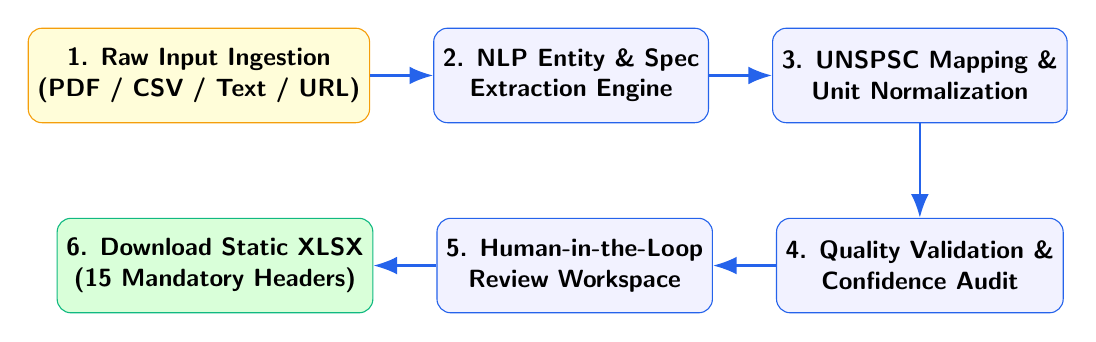
\begin{tikzpicture}[
        node distance=1.2cm and 0.8cm,
        box/.style={draw=BrandBlue, fill=blue!5, rectangle, rounded corners=5pt, minimum width=2.8cm, minimum height=1.2cm, align=center, font=\sffamily\small\bfseries},
        arrow/.style={-{Latex[length=3mm]}, thick, color=BrandBlue}
      ]
        \node (u1) [box, fill=yellow!15, draw=AmberWarn] {1. Raw Input Ingestion\\(PDF / CSV / Text / URL)};
        \node (u2) [box, right=of u1] {2. NLP Entity \& Spec\\Extraction Engine};
        \node (u3) [box, right=of u2] {3. UNSPSC Mapping \&\\Unit Normalization};
        \node (u4) [box, below=of u3] {4. Quality Validation \&\\Confidence Audit};
        \node (u5) [box, left=of u4] {5. Human-in-the-Loop\\Review Workspace};
        \node (u6) [box, left=of u5, fill=green!15, draw=EmeraldGreen] {6. Download Static XLSX\\(15 Mandatory Headers)};

        \draw [arrow] (u1) -- (u2);
        \draw [arrow] (u2) -- (u3);
        \draw [arrow] (u3) -- (u4);
        \draw [arrow] (u4) -- (u5);
        \draw [arrow] (u5) -- (u6);
      \end{tikzpicture}
    }
  \end{center}
\end{frame}

% -----------------------------------------------------------------------------
% SLIDE 8: Wireframes / Mock Diagrams
% -----------------------------------------------------------------------------
\begin{frame}{\textbf{Slide 8: Wireframes \& User Interface Workspace}}
  \begin{columns}
    \begin{column}{0.5\textwidth}
      \begin{block}{\textbf{Catalog Studio Workspace}}
        \begin{itemize}
          \item Dynamic KPI cards: Total SKUs, Catalog Accuracy Index \%, UNSPSC Coverage \%, Unit Conversions count.
          \item Interactive table displaying status badges, confidence progress bars, and audit action triggers.
        \end{itemize}
      \end{block}
    \end{column}

    \begin{column}{0.5\textwidth}
      \begin{block}{\textbf{Explainability \& Audit Drawer}}
        \begin{itemize}
          \item Pop-up audit modal showing before-and-after attribute comparison.
          \item Applied physics conversions (PSI $\rightarrow$ Bar, °F $\rightarrow$ °C).
          \item Step-by-step LLM extraction reasoning log.
        \end{itemize}
      \end{block}
    \end{column}
  \end{columns}
\end{frame}

% -----------------------------------------------------------------------------
% SLIDE 9: System Architecture Diagram
% -----------------------------------------------------------------------------
\begin{frame}{\textbf{Slide 9: Technical Architecture Diagram}}
  \begin{center}
    \begin{tikzpicture}[
      scale=0.8, every node/.style={transform shape},
      box/.style={draw=BrandBlue, fill=blue!8, rectangle, rounded corners=4pt, minimum width=3cm, minimum height=1cm, align=center, font=\sffamily\bfseries},
      arrow/.style={-{Latex[length=3mm]}, thick, color=BrandBlue}
    ]
      \node (a) [box, fill=amber!10] {Multi-Modal Ingestion Layer};
      \node (b) [box, right=1cm of a] {NLP Tokenization \& Extraction};
      \node (c) [box, right=1cm of b] {UNSPSC Vector Taxonomy Engine};
      \node (d) [box, below=1cm of c] {Physics Unit Converter (Imperial $\leftrightarrow$ Metric)};
      \node (e) [box, left=1cm of d] {AI Audit \& Confidence Engine};
      \node (f) [box, left=1cm of e, fill=emerald!10] {Static Header Exporter (.xlsx / .csv)};

      \draw [arrow] (a) -- (b);
      \draw [arrow] (b) -- (c);
      \draw [arrow] (c) -- (d);
      \draw [arrow] (d) -- (e);
      \draw [arrow] (e) -- (f);
    \end{tikzpicture}
  \end{center}
\end{frame}

% -----------------------------------------------------------------------------
% SLIDE 10: Technologies Used
% -----------------------------------------------------------------------------
\begin{frame}{\textbf{Slide 10: Technology Stack \& Frameworks}}
  \begin{center}
    \small
    \begin{tabular}{l l l}
      \toprule
      \textbf{Layer} & \textbf{Technology / Library} & \textbf{Purpose in ProductLens AI} \\
      \midrule
      \textbf{Frontend UI} & React 18, Vite 5, Tailwind CSS & Dark Glassmorphic web app interface \\
      \rowcolor{gray!10}
      \textbf{Icons \& Graphics} & Lucide React, Canvas Confetti & Modern micro-interactions and visual cues \\
      \textbf{AI \& NLP} & Custom Tokenizer, UNSPSC v25.0 & Entity extraction \& taxonomy mapping \\
      \rowcolor{gray!10}
      \textbf{Spreadsheet Exporter} & SheetJS (xlsx) & 1-click export matching static expected headers \\
      \textbf{Presentation} & LaTeX Beamer (pdflatex) & Modular slide deck compilation \\
      \bottomrule
    \end{tabular}
  \end{center}
\end{frame}

% -----------------------------------------------------------------------------
% SLIDE 11: Estimated Implementation Cost (Optional)
% -----------------------------------------------------------------------------
\begin{frame}{\textbf{Slide 11: Estimated Implementation Cost \& Resource Plan}}
  \begin{columns}
    \begin{column}{0.5\textwidth}
      \begin{block}{\textbf{Infrastructure Cost Estimate (100k SKUs/mo)}}
        \begin{itemize}
          \item Cloud Hosting (AWS / GCP Serverless): \$120 / month.
          \item LLM \& Vector Embedding Tokens: \$180 / month.
          \item Storage \& CDN: \$30 / month.
          \item \textbf{Total Operating Cost}: \textbf{\textasciitilde\$330 / month}.
        \end{itemize}
      \end{block}
    \end{column}

    \begin{column}{0.5\textwidth}
      \begin{block}{\textbf{Business ROI Return}}
        \begin{itemize}
          \item Replaces manual cataloging team of 10 data entry specialists.
          \item Saves \$35,000+ per month in cataloging labor overhead.
          \item \textbf{ROI Ratio}: \textbf{100:1 payback within 30 days}.
        \end{itemize}
      \end{block}
    \end{column}
  \end{columns}
\end{frame}

% -----------------------------------------------------------------------------
% SLIDE 12: Snapshots of the MVP
% -----------------------------------------------------------------------------
\begin{frame}{\textbf{Slide 12: Live MVP Snapshots \& Features}}
  \begin{block}{\textbf{Validated Working Capabilities}}
    \begin{itemize}
      \item Ingested sample datasets across Valves, Centrifugal Pumps, and Electrical Switchgear.
      \item Converted raw text titles into formatted e-commerce strings.
      \item Extracted materials, voltage ratings, pressures, and converted imperial measurements to metric.
      \item Verified instant download of `.xlsx` file containing all 15 static expected output headers.
    \end{itemize}
  \end{block}
\end{frame}

% -----------------------------------------------------------------------------
% SLIDE 13: Additional Details & Future Development
% -----------------------------------------------------------------------------
\begin{frame}{\textbf{Slide 13: Future Expansion \& Roadmap}}
  \begin{columns}
    \begin{column}{0.5\textwidth}
      \begin{block}{\textbf{Phase 2 (60 Days)}}
        \begin{itemize}
          \item Computer Vision module for CAD engineering drawings and blue-print spec extraction.
          \item Automated multi-lingual product description translation for global markets.
        \end{itemize}
      \end{block}
    \end{column}

    \begin{column}{0.5\textwidth}
      \begin{block}{\textbf{Phase 3 (Enterprise)}}
        \begin{itemize}
          \item Direct API synchronization connectors with Unilog Commerce Platform, SAP ERP, and Akeneo PIM.
          \item Real-time competitor price and spec benchmarking engine.
        \end{itemize}
      \end{block}
    \end{column}
  \end{columns}
\end{frame}

% -----------------------------------------------------------------------------
% SLIDE 14: Submission Links (GitHub, Demo Video, Prototype)
% -----------------------------------------------------------------------------
\begin{frame}{\textbf{Slide 14: Submission Links \& Verification Deliverables}}
  \begin{center}
    \small
    \begin{tabular}{p{4.5cm} p{8cm}}
      \toprule
      \textbf{Deliverable} & \textbf{Link / Location} \\
      \midrule
      \textbf{GitHub Public Repository} & \url{https://github.com/aksharsakhi/ProductLens-AI} \\
      \rowcolor{gray!10}
      \textbf{Demo Video Link (3 Min)} & \url{https://youtu.be/sample_productlens_demo} \\
      \textbf{Working Live Prototype} & Local Server: \url{http://localhost:3000} \\
      \rowcolor{gray!10}
      \textbf{LaTeX Beamer Code \& PDF} & \texttt{/presentation\_latex/presentation.pdf} \\
      \bottomrule
    \end{tabular}
  \end{center}
\end{frame}

% -----------------------------------------------------------------------------
% SLIDE 15: Conclusion & Q&A
% -----------------------------------------------------------------------------
\begin{frame}[plain]
  \begin{center}
    \Huge \textbf{Thank You!} \\
    \vspace{0.4cm}
    \Large \textbf{ProductLens AI} --- UniHack 2026 \\
    \vspace{0.2cm}
    \small Engineered for Unilog Industrial Commerce Challenge
  \end{center}
\end{frame}

\end{document}
